\chapter{ Констукторский раздел}
\label{cha:design}
    В данном разделе будут рассмотрены схемы алгоритмов, требования к функциональности ПО,
    и опредены способы тестирования.
    
    \section{Разработка алгоритмов}
        Ниже будут представлены схемы алгоритмов поиска: \begin{enumerate}
            \item алгоритм поиска полным перебором (рисунок \ref{schema:search:brute-force});
            \item алгоритм двоичного поиска  (рисунок \ref{schema:search:binary});
            \item алгоритм поиска по сегментам (рисунок \ref{schema:search:segment}).
        \end{enumerate}

    \begin{figure}[h!]
        \centering
            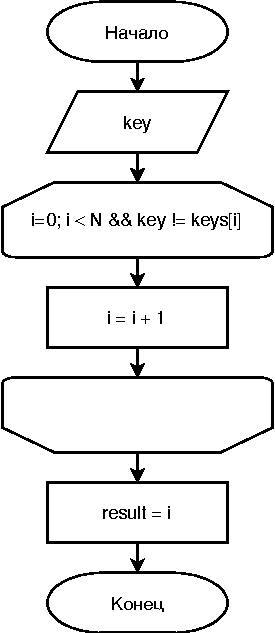
\includegraphics[scale=0.9]{schema_brute_force.pdf}
            \caption{Схема алгоритма поиска полным перебором}
            \label{schema:search:brute-force}
    \end{figure}

    \begin{figure}[h!]
        \centering
            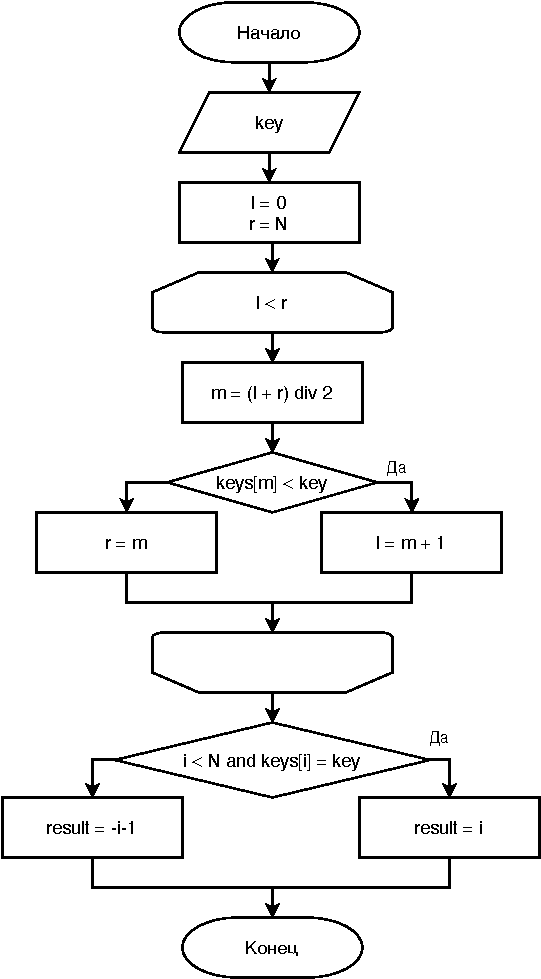
\includegraphics[scale=0.9]{schema_binary_search.pdf}
            \caption{Схема алгоритма бинарного поиска}
            \label{schema:search:binary}
    \end{figure}

    \begin{figure}[h!]
        \centering
            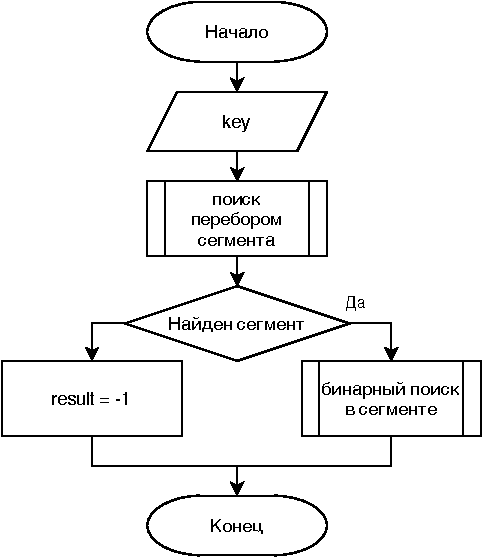
\includegraphics[scale=0.9]{schema_segment_search.pdf}
            \caption{Схема алгоритма поиска по сегментам}
            \label{schema:search:segment}
    \end{figure}

    \section{Требования к функциональности ПО}
        В данной работе требуется обеспечить следующую минимальную функциональность консольного приложения:
        \begin{enumerate}
            \item загрузка словаря из текстового файла;
            \item вывод замеров времени работы каждого из алгоритмов в текстовый файл.
        \end{enumerate}

    \section{Тестирование}
        Тестирование ПО будет проводиться методом чёрного ящика. Необходимо проверить работу системы 
        на случаях, когда словарь является пустым, содержит один и более элементов.

\newpage